\documentclass{standalone}

\usepackage{tikz}
\usetikzlibrary{automata, arrows.meta, positioning, shapes}

\begin{document}
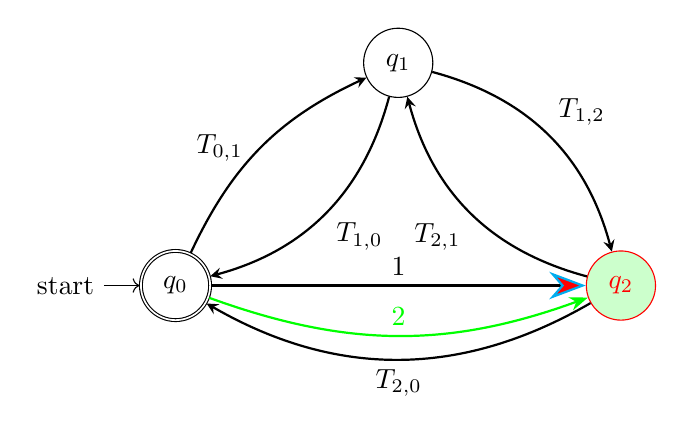
\begin{tikzpicture} [node distance = 4cm, on grid, auto]

\node (q0) [state, initial, accepting, initial text = {start}] {$q_0$};
\node (q1) [state, above right = of q0] {$q_1$};
\node (q2) [state, below right = of q1, color=red, fill=green!20] {$q_2$};

\path [-stealth, thick]
    (q0) edge [bend left=20] node [left=0.1cm]  {$T_{0,1}$} (q1)
    (q1) edge [bend left]    node [above right] {$T_{1,2}$} (q2)
         edge [bend left]    node [below right] {$T_{1,0}$} (q0)
    (q2) edge [bend left=30] node [below]       {$T_{2,0}$} (q0)
    (q2) edge [bend left]    node [below left]  {$T_{2,1}$} (q1);

\path [-{Stealth[scale=2, color=cyan, fill=red]}, thick]
    (q0) edge node {1} (q2);

\path [green, -Stealth, thick]
    (q0) edge [bend right=20] node {2} (q2);

\end{tikzpicture}
\end{document}
